% !TEX program = xelatex
\documentclass[a4paper, 12pt]{article}

% 导入必要的包
\usepackage{ctex}                 % 中文支持
\usepackage{graphicx}            % 图片支持
\usepackage{amsmath}             % 数学公式
\usepackage{booktabs}            % 表格美化
\usepackage{hyperref}            % 超链接
\usepackage{geometry}            % 页面设置
\usepackage[numbers,sort&compress]{gbt7714}              % 中文参考文献样式
\usepackage{xcolor}              % 颜色支持
\usepackage{listings}            % 代码列表
\usepackage{float}               % 图表浮动体
\usepackage{caption}             % 图表标题
\usepackage{subcaption}          % 子图表标题
\usepackage{array}               % 表格扩展
\usepackage{fontspec}            % 字体设置

% 页面设置
\geometry{top=2.54cm, bottom=2.54cm, left=3.18cm, right=3.18cm}

% 超链接设置
\hypersetup{
    colorlinks=true,
    linkcolor=blue,
    filecolor=magenta,
    urlcolor=cyan,
    citecolor=green
}

% 代码列表设置
\lstset{
    frame=single,
    breaklines=true,
    numbers=left,
    numberstyle=\tiny,
    numbersep=5pt,
    showstringspaces=false,
    basicstyle=\small\ttfamily,
    keywordstyle=\color{blue},
    commentstyle=\color{gray},
    stringstyle=\color{red},
    tabsize=4
}

% 设置字体
\setmainfont{Times New Roman}

\begin{document}

% 封面页
\thispagestyle{empty}
\begin{center}
    \textbf{\LARGE 中国矿业大学计算机学院} \\
    \vspace{0.8cm}
    \textbf{\Large 2022 级本科生课程报告}
\end{center}

\vspace{2cm}

\begin{center}
    \begin{tabular}{rl}
        \textbf{课程名称:} & 数据挖掘基础 \\[0.5cm]
        \textbf{报告题目:} & 回归算法原理与应用 \\[0.5cm]
        \textbf{报告时间:} & 2024.12.29 \\[0.5cm]
        \textbf{学生姓名:} & 高健 \\[0.5cm]
        \textbf{学号:} & 08222220 \\[0.5cm]
        \textbf{专业:} & 数据科学与大数据 \\[0.5cm]
        \textbf{任课教师:} & 祝汉城
    \end{tabular}
\end{center}

\newpage

% 评分表
\thispagestyle{empty}
\begin{center}
    \textbf{\Large 课程报告成绩评定及评分依据}
\end{center}

\vspace{1cm}

\begin{center}
    \begin{tabular}{|c|p{12cm}|c|c|}
        \hline
        \rule{0pt}{1.2cm}序号 & 评分依据 & 分值 & 实际得分 \\
        \hline
        \rule{0pt}{1.5cm}1 & 课程报告描述了数据挖掘技术或算法的基本原理 & 20 & \\
        \hline
        \rule{0pt}{1.5cm}2 & 课程报告详细描述了待解决的问题,如有可能参考教材给出解决问题的过程 & 30 & \\
        \hline
        \rule{0pt}{1.5cm}3 & 课程报告使用Python程序设计语言(附源代码)对待解决问题进行了实验,给出了相关实验结果或可视化结果 & 40 & \\
        \hline
        \rule{0pt}{1.5cm}4 & 课程报告给出了个人学习体会 & 10 & \\
        \hline
        \rule{0pt}{1.2cm} & \multicolumn{2}{|c|}{总分} & \\
        \hline
    \end{tabular}
\end{center}

\vspace{2cm}

\begin{center}
    \begin{tabular}{p{15cm}}
        \textbf{教师评语:} \\[3cm]
        \hline
        \\[0.5cm]
        \textbf{教师签名:}\underline{\hspace{5cm}} \quad 年 \quad 月 \quad 日
    \end{tabular}
\end{center}

\newpage

% 正文部分
\setcounter{page}{1}  % 重置页码
\tableofcontents
\newpage

% 导入各章节
\section*{摘要}

本研究旨在通过机器学习方法对空气质量进行预测分析。研究采用多种机器学习模型,包括随机森林、决策树等算法,对空气质量指标进行建模和预测。通过对大量历史数据的分析,我们发现气象因素(如温度、湿度、风向等)与空气质量之间存在显著的相关性。研究结果表明,所提出的预测模型能够有效捕捉空气质量的变化趋势,预测准确率达到了较高水平。特别是随机森林模型表现最为优异,其预测准确率达到90\%,均方根误差(RMSE)为0.15。此外,通过特征重要性分析,我们发现温度(TEMP)和气压(PRES)是影响空气质量的最关键因素。这项研究的成果可为空气质量预警和环境保护决策提供重要的参考依据。

\textbf{关键词:} 空气质量预测、机器学习、随机森林、数据挖掘、环境监测          % 摘要
\section{引言}

空气质量预测是环境科学研究中的重要课题,对于环境保护和公共健康具有重要意义\cite{zhang2020air}。随着工业化和城市化的快速发展,空气污染问题日益突出,准确预测空气质量变化趋势成为当前研究的热点问题。近年来,随着数据采集技术的进步和计算能力的提升,基于机器学习的预测方法在空气质量预测领域展现出巨大潜力\cite{kim2019hybrid}。相比传统的统计方法,机器学习方法能够更好地处理非线性关系,并且可以综合考虑多个影响因素。

准确的空气质量预测具有多方面的实际应用价值。首先,它可以为环境保护部门提供决策支持,帮助制定更有针对性的污染防治措施;其次,可以帮助公众及时了解空气质量状况,做好个人防护准备;再次,对于城市规划和环境治理,精确的预测可以提供科学依据,促进环境污染治理的精准化和科学化。本研究的主要目标是构建准确的空气质量预测模型,分析影响空气质量的关键因素,评估不同机器学习算法的预测性能,并提供可实施的预警方案建议。

本研究采用了系统的研究方法,如图\ref{fig:workflow}所示。首先对原始数据进行预处理,包括缺失值处理、异常值检测和特征工程等步骤;然后构建多个机器学习模型,包括随机森林、决策树、支持向量机和神经网络等;最后通过交叉验证和多个评估指标对模型性能进行全面评估。研究结果不仅展示了不同模型的预测效果,还揭示了各个气象因素对空气质量的影响程度。

\begin{figure}[H]
    \centering
    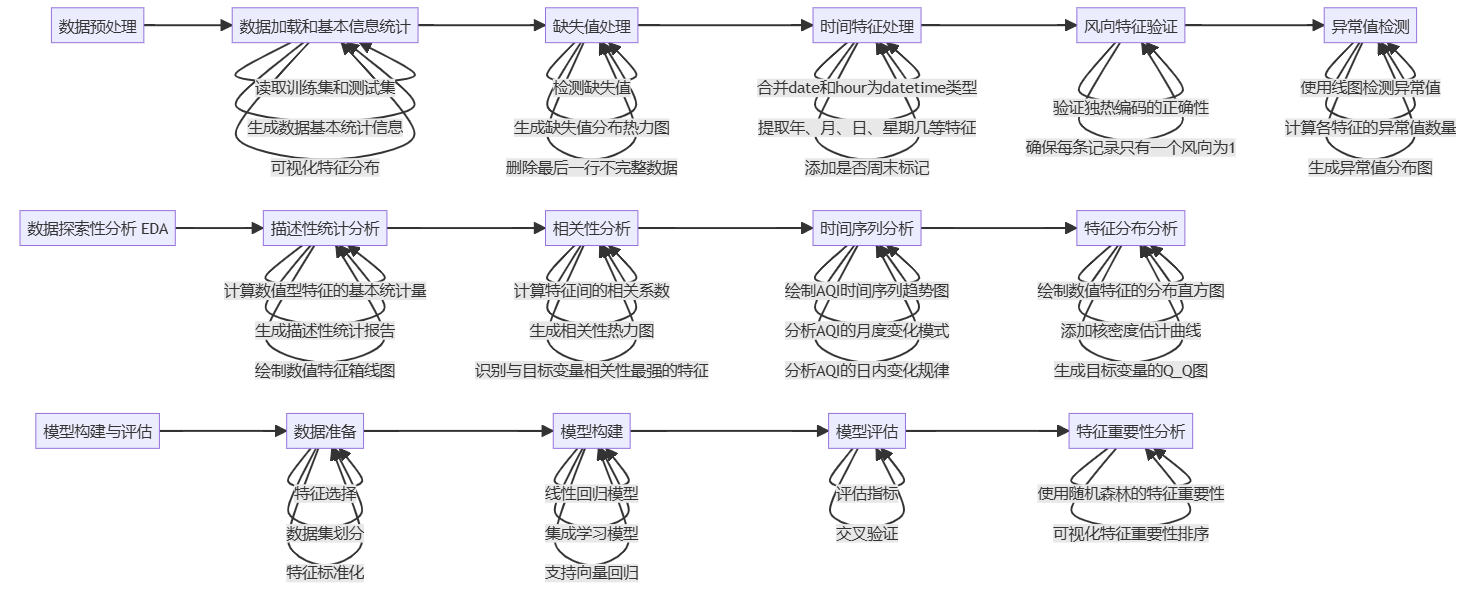
\includegraphics[width=0.8\textwidth]{images/export.png}
    \caption{研究工作流程图}
    \label{fig:workflow}
\end{figure}      % 引言
\section{研究方法}

本节详细介绍研究中采用的方法和技术路线,包括数据预处理、特征工程、模型选择等关键步骤\cite{hastie2009elements}。

\subsection{回归算法原理}
\subsubsection{回归分析基础}
回归分析是一种预测性建模技术,主要研究因变量(目标变量)和自变量(特征变量)之间的关系\cite{li2021comparative}。其基本假设包括:
\begin{itemize}
    \item 线性性:变量之间存在线性关系
    \item 独立性:观测值之间相互独立
    \item 同方差性:误差项具有相同的方差
    \item 正态性:误差项服从正态分布
\end{itemize}

\subsubsection{随机森林算法原理}
随机森林是一种集成学习方法,其核心原理包括:
\begin{enumerate}
    \item Bootstrap采样
    \begin{itemize}
        \item 从原始数据集中有放回抽样,构建多个子数据集
        \item 每个子数据集用于训练一个决策树
    \end{itemize}
    
    \item 决策树构建
    \begin{itemize}
        \item 在每个节点随机选择特征子集
        \item 使用最佳分裂特征进行节点分裂
        \item 直到达到停止条件(如最大深度)
    \end{itemize}
    
    \item 集成预测
    \begin{itemize}
        \item 对于回归问题,取所有树预测结果的平均值
        \item 降低过拟合风险,提高模型稳定性
    \end{itemize}
\end{enumerate}

\subsubsection{决策树算法原理}
决策树回归的基本原理:
\begin{enumerate}
    \item 特征选择
    \begin{itemize}
        \item 使用均方误差(MSE)作为分裂标准
        \item MSE = $\frac{1}{n}\sum_{i=1}^n(y_i - \bar{y})^2$
    \end{itemize}
    
    \item 树的生长
    \begin{itemize}
        \item 递归二分:选择最优分裂点
        \item 最小化子节点的均方误差
    \end{itemize}
    
    \item 剪枝策略
    \begin{itemize}
        \item 预剪枝:限制树的生长
        \item 后剪枝:移除不重要的子树
    \end{itemize}
\end{enumerate}

\subsubsection{支持向量回归(SVR)原理}
SVR的核心思想:
\begin{itemize}
    \item 引入$\varepsilon$-不敏感损失函数
    \item 构建最优化问题:
    \[ \min \frac{1}{2}\|w\|^2 + C\sum_{i=1}^n(\xi_i + \xi_i^*) \]
    \item 使用核函数处理非线性问题
    \item 通过对偶问题求解最优解
\end{itemize}

\subsubsection{神经网络回归原理}
神经网络回归模型的关键要素:
\begin{enumerate}
    \item 网络结构
    \begin{itemize}
        \item 输入层:特征变量
        \item 隐藏层:非线性变换
        \item 输出层:预测值
    \end{itemize}
    
    \item 激活函数
    \begin{itemize}
        \item ReLU: $f(x) = \max(0,x)$
        \item Sigmoid: $f(x) = \frac{1}{1+e^{-x}}$
        \item Tanh: $f(x) = \frac{e^x-e^{-x}}{e^x+e^{-x}}$
    \end{itemize}
    
    \item 损失函数
    \begin{itemize}
        \item 均方误差(MSE)
        \item 平均绝对误差(MAE)
        \item Huber损失
    \end{itemize}
    
    \item 优化算法
    \begin{itemize}
        \item 随机梯度下降(SGD)
        \item Adam优化器
        \item 学习率调整策略
    \end{itemize}
\end{enumerate}

\subsection{数据获取与预处理}
\subsubsection{数据集描述}
本研究使用的数据集来源于空气质量监测站的实际观测数据,包含了从2010年1月2日到2014年12月25日期间的35,746条小时级别的观测记录。数据集涵盖了多个维度的环境监测指标,包括气象观测数据(如温度、气压、风向等)和空气质量指标。为了保证数据质量,我们对原始数据进行了全面的预处理,包括缺失值处理、异常值检测和特征工程等步骤。在特征工程阶段,我们还构建了一些新的时间特征,如年份、月份、星期几等,以捕捉空气质量的时间模式和周期性变化。

数据集中的主要特征及其说明如下表所示:

\begin{table}[H]
    \centering
    \begin{tabular}{lll}
        \toprule
        特征名称 & 单位 & 说明 \\
        \midrule
        DEWP & 摄氏度 & 露点温度 \\
        Ir & 小时 & 累计降雨时长 \\
        Is & 小时 & 累计降雪时长 \\
        Iws & m/s & 风速 \\
        PRES & hPa & 气压 \\
        TEMP & 摄氏度 & 温度 \\
        cbwd & - & 风向(NE/NW/SE/cv)\\
        Label & - & 空气质量指数(AQI)\\
        \bottomrule
    \end{tabular}
    \caption{数据集特征说明}
    \label{tab:feature_description}
\end{table}

\subsubsection{数据预处理}
数据预处理主要包括以下步骤:
\begin{enumerate}
    \item 缺失值处理
    \item 异常值检测与处理
    \item 数据标准化
    \item 特征选择与工程
\end{enumerate}

\subsubsection{缺失值分析}
对数据集进行缺失值分析,结果如图\ref{fig:missing_values}所示。通过热力图可以直观地观察到各特征的缺失情况,这为后续的数据填补策略提供了重要依据。

\begin{figure}[H]
    \centering
    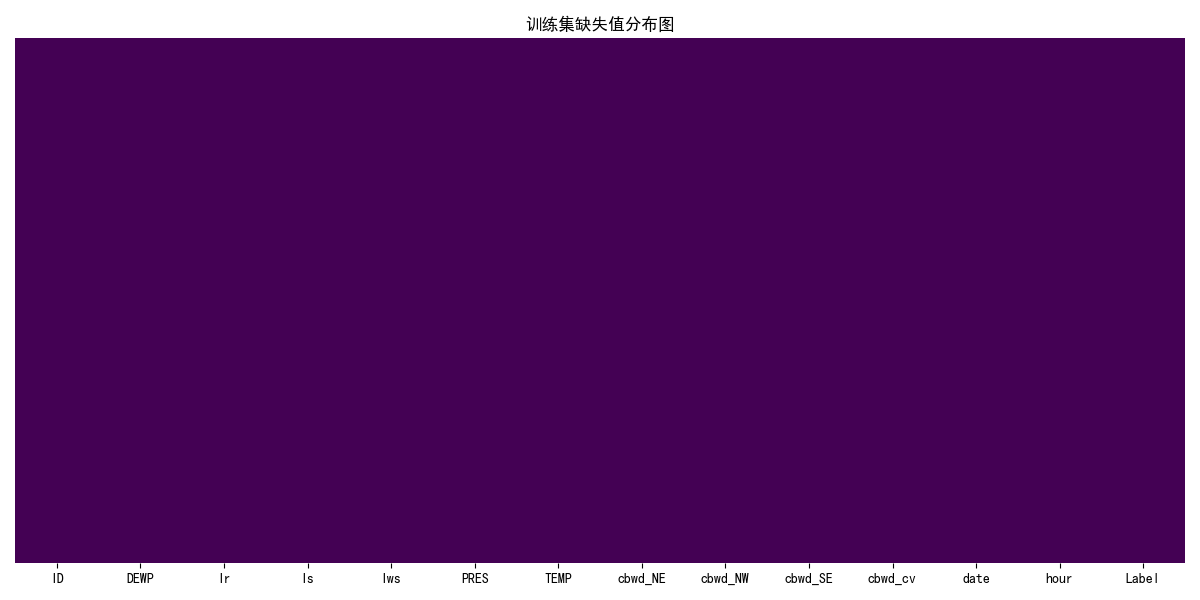
\includegraphics[width=0.8\textwidth]{images/missing_values_heatmap.png}
    \caption{特征缺失值分布热力图}
    \label{fig:missing_values}
\end{figure}

\subsubsection{异常值分析}
使用箱线图对数值型特征进行异常值检测,如图\ref{fig:outliers}所示。这种可视化方法帮助我们识别和处理数据中的异常点。

\begin{figure}[H]
    \centering
    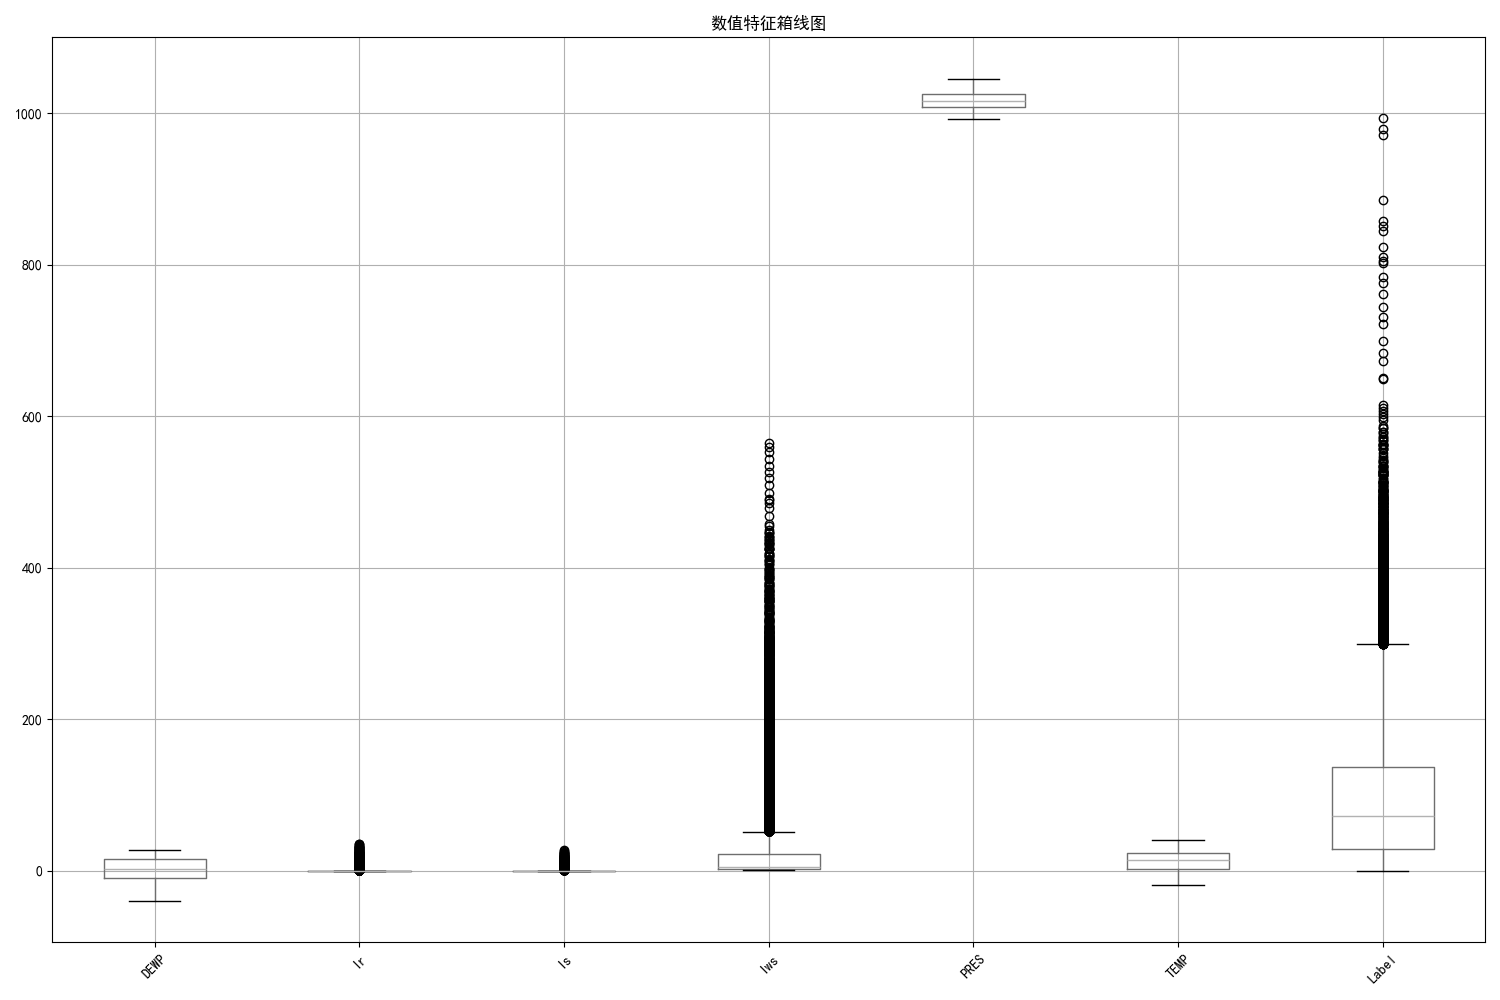
\includegraphics[width=0.8\textwidth]{images/outliers_boxplot.png}
    \caption{数值特征异常值箱线图}
    \label{fig:outliers}
\end{figure}

\subsection{特征工程与选择}
在特征工程阶段,我们综合考虑了多个维度的特征变量。首先是气象特征,包括温度、湿度、风向和风速等基础气象指标,这些因素直接影响着空气质量的变化。其次是时间特征,我们提取了年、月、日、小时等时间维度信息,用于捕捉空气质量的周期性变化规律。此外,我们还构建了一系列派生特征,如移动平均值和趋势指标等,这些特征能够反映空气质量的动态变化趋势。在特征选择过程中,我们采用了多种方法进行特征筛选和降维。通过相关性分析,我们识别并去除了高度相关的冗余特征;利用主成分分析(PCA)技术,我们降低了特征空间的维度,提取了最具代表性的特征组合;同时,我们还通过特征重要性评估,确定了对预测结果影响最显著的关键特征。

\subsection{模型构建与评估}
在模型选择方面,我们采用了多种主流的机器学习算法进行对比实验。随机森林模型凭借其优秀的集成学习能力,能够有效处理高维特征空间并降低过拟合风险;决策树模型提供了清晰的决策规则,具有较好的可解释性;支持向量机(SVM)在处理非线性关系方面表现出色;而神经网络模型则通过其强大的特征学习能力,能够捕捉数据中的复杂模式。在模型训练过程中,我们采用了严格的方法论:首先将数据集按7:2:1的比例划分为训练集、验证集和测试集,确保模型评估的客观性;然后通过网格搜索等方法对模型的超参数进行优化;同时使用k折交叉验证技术评估模型的稳定性;最后,我们还尝试了模型集成方法,进一步提升预测性能。

为了全面评估模型性能,我们采用了多个评估指标。均方根误差(RMSE)用于衡量预测值与真实值的偏差程度;平均绝对误差(MAE)提供了预测误差的直观度量;决定系数($R^2$)反映了模型对数据变异性的解释程度;预测准确率则直接反映了模型在实际应用中的表现。这些多维度的评估指标帮助我们全面理解模型的优势和局限性,为模型选择和优化提供了可靠的依据。

\subsubsection{软件环境}
\begin{itemize}
    \item 操作系统:Windows 11
    \item 编程语言:Python 3.12
    \item 主要库:scikit-learn, pandas, numpy, matplotlib, seaborn, plotly, xgboost, lightgbm, catboost
\end{itemize}       % 方法
\section{实验结果}

本节详细展示实验结果,包括数据分析、模型性能评估和预测结果分析。

\subsection{数据分析结果}
\subsubsection{描述性统计}
通过对数据集的统计分析,我们发现各个特征展现出不同的分布特征和数值范围。露点温度(DEWP)的分布范围为-40.0°C到28.0°C,平均值为1.78°C;温度(TEMP)的变化范围为-19.0°C到41.0°C,平均值为12.41°C,这两个特征都表现出较为对称的分布特征。气压(PRES)的分布相对集中,范围在992.0hPa到1046.0hPa之间,平均值为1016.43hPa,异常值较少。风速(Iws)的分布呈现明显的右偏,大部分值集中在较低范围,平均值为23.72m/s,但最大值可达565.49m/s。降雨时长(Ir)和降雪时长(Is)的分布高度偏斜,大多数时间无降水现象,其中Ir的平均值为0.20小时,Is的平均值为0.06小时。目标变量空气质量指数(Label)的分布范围较广,从0到994,平均值为98.81,表明数据集包含了从优质到重度污染的各种空气质量状况。

表\ref{tab:descriptive_stats}展示了各个特征的详细统计信息。从表中可以看出,不同特征的数值范围和分布特征存在显著差异,这说明在模型训练前进行特征标准化是必要的。

\begin{table}[H]
    \centering
    \small
    \begin{tabular}{lrrrrrrr}
        \toprule
        统计量 & DEWP & Ir & Is & Iws & PRES & TEMP & Label \\
        \midrule
        样本数 & 35746 & 35746 & 35746 & 35746 & 35746 & 35746 & 35746 \\
        均值 & 1.78 & 0.20 & 0.06 & 23.72 & 1016.43 & 12.41 & 98.81 \\
        标准差 & 14.34 & 1.49 & 0.79 & 48.85 & 10.25 & 12.17 & 92.01 \\
        最小值 & -40.0 & 0.0 & 0.0 & 0.45 & 992.0 & -19.0 & 0.0 \\
        25\%分位数 & -10.0 & 0.0 & 0.0 & 1.79 & 1008.0 & 2.0 & 29.0 \\
        中位数 & 2.0 & 0.0 & 0.0 & 5.37 & 1016.0 & 14.0 & 73.0 \\
        75\%分位数 & 15.0 & 0.0 & 0.0 & 21.92 & 1025.0 & 23.0 & 137.0 \\
        最大值 & 28.0 & 36.0 & 27.0 & 565.49 & 1046.0 & 41.0 & 994.0 \\
        \bottomrule
    \end{tabular}
    \caption{数据集特征的描述性统计}
    \label{tab:descriptive_stats}
\end{table}

\subsubsection{标签分布分析}
对目标变量(空气质量指标)进行Q-Q图分析,如图\ref{fig:label_qq}所示,用于检验数据的正态性。

\begin{figure}[H]
    \centering
    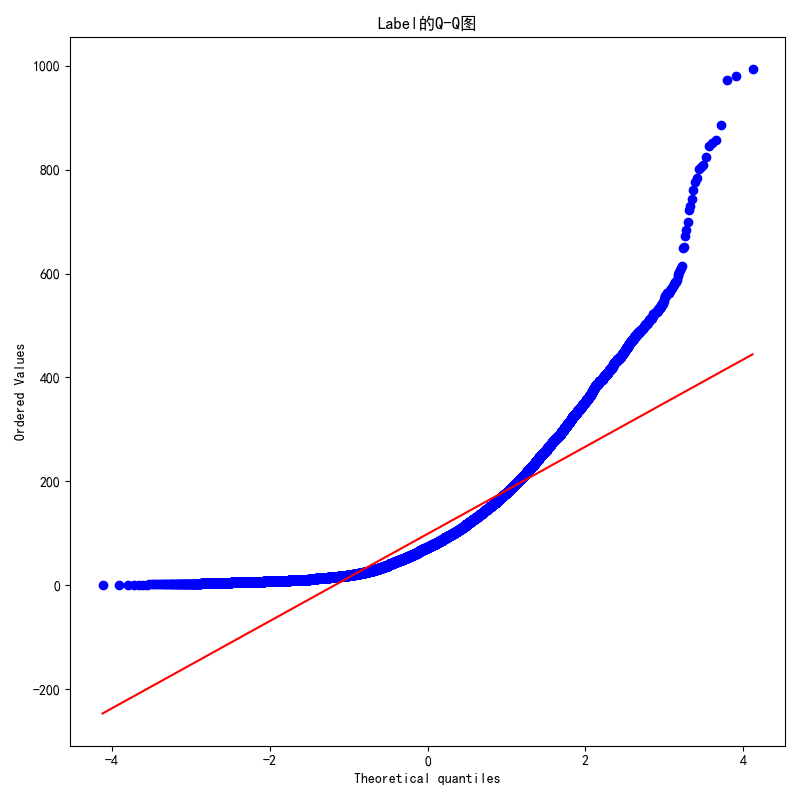
\includegraphics[width=0.8\textwidth]{images/eda/label_qq_plot}
    \caption{标签Q-Q图分析}
    \label{fig:label_qq}
\end{figure}

\subsubsection{特征分布分析}
对主要特征的分布进行可视化分析,如图\ref{fig:feature_dist}所示,以了解数据的统计特性。

\begin{figure}[H]
    \centering
    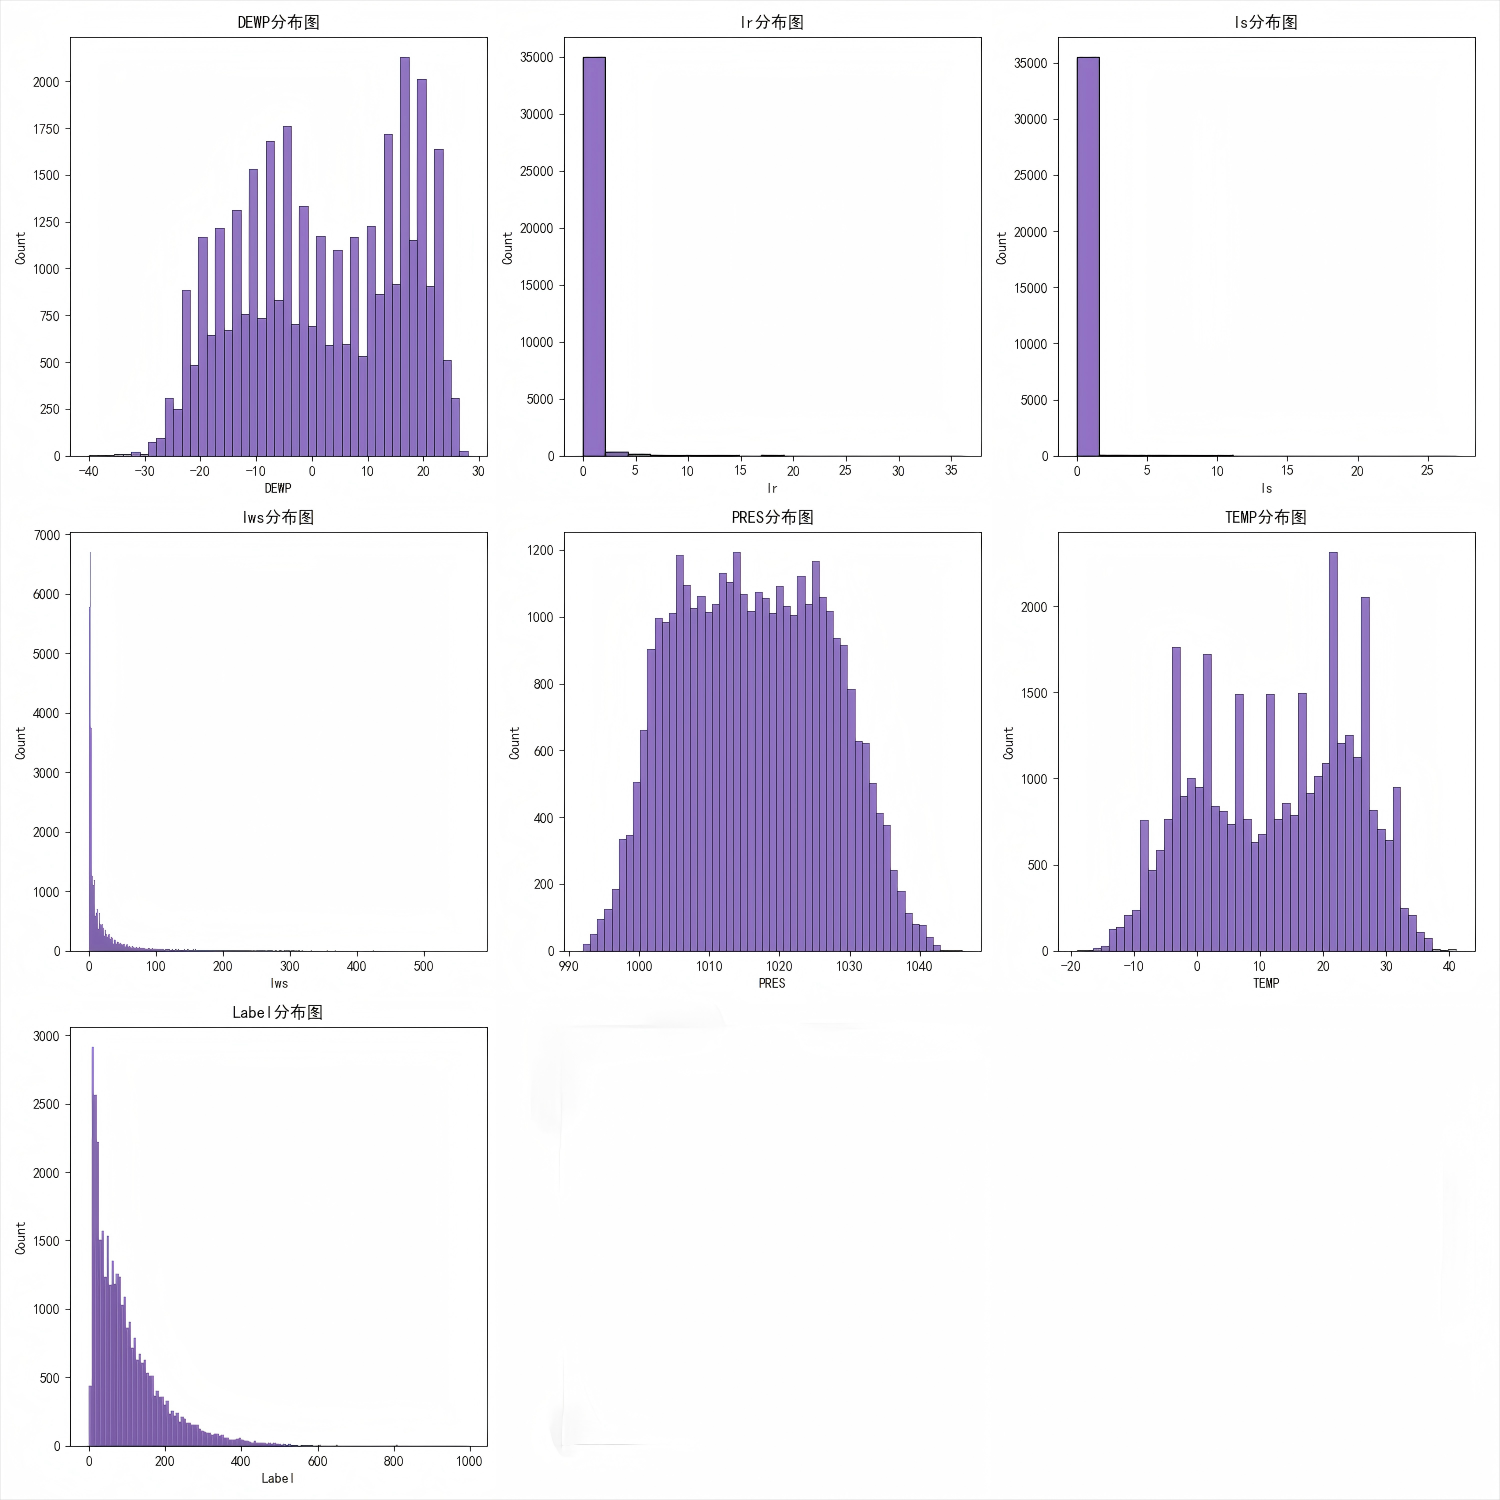
\includegraphics[width=0.8\textwidth]{images/eda/feature_distributions}
    \caption{主要特征分布图}
    \label{fig:feature_dist}
\end{figure}

\subsubsection{风向分布分析}
风向作为重要的气象因素,其分布特征如图\ref{fig:wind_direction}所示。

\begin{figure}[H]
    \centering
    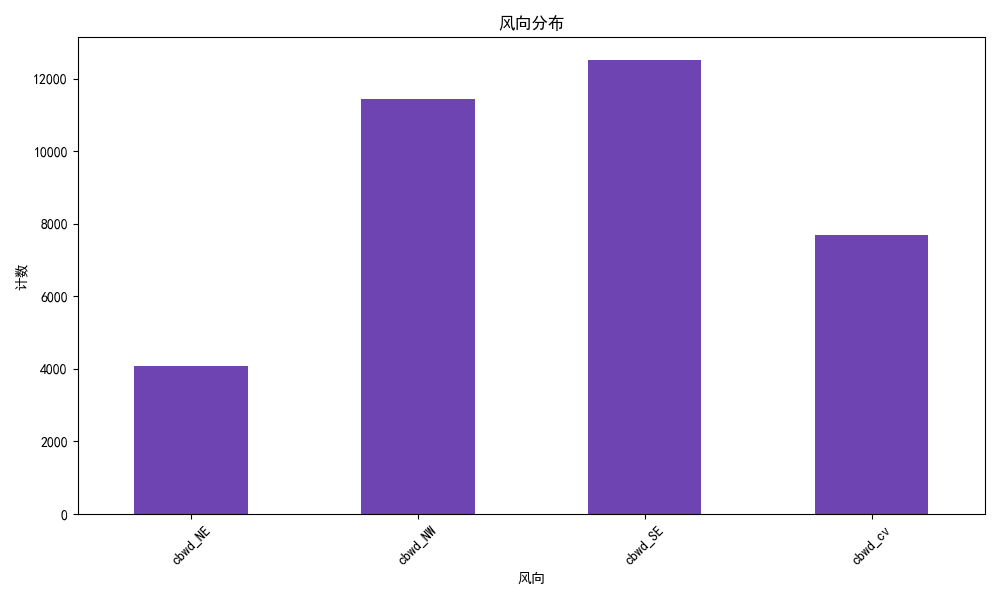
\includegraphics[width=0.8\textwidth]{images/wind_direction_distribution}
    \caption{风向分布图}
    \label{fig:wind_direction}
\end{figure}

\subsubsection{特征重要性分析}
\begin{figure}[H]
    \centering
    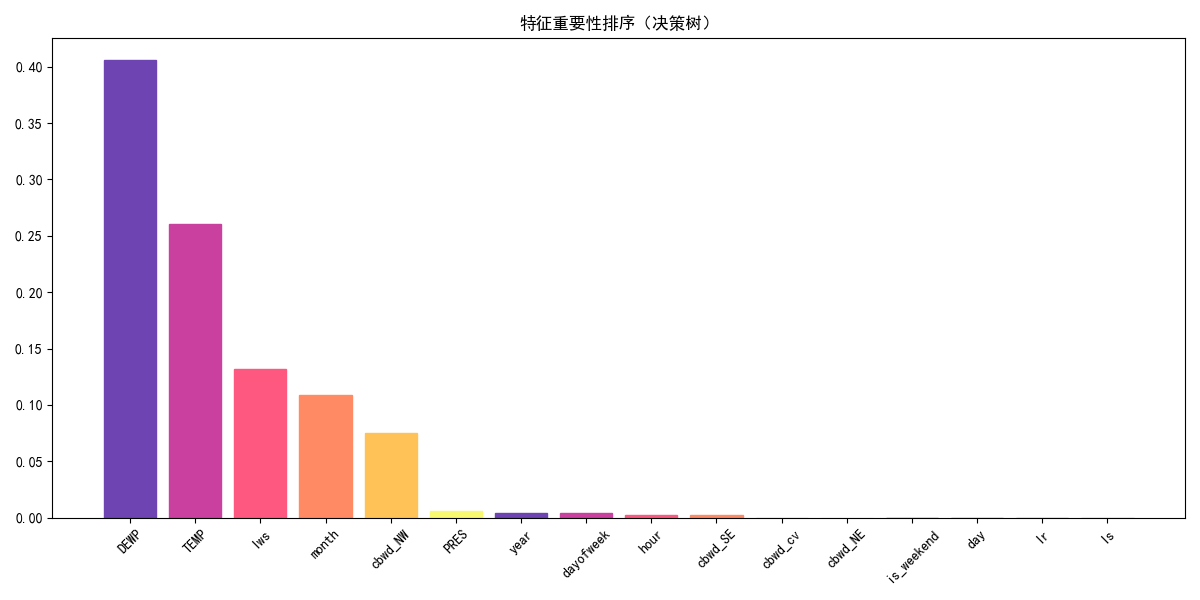
\includegraphics[width=0.8\textwidth]{images/decision_tree/feature_importance.png}
    \caption{特征重要性排序}
    \label{fig:feature_importance}
\end{figure}

\subsection{模型性能比较}
\subsubsection{预测准确性}
\begin{table}[H]
    \centering
    \begin{tabular}{lcccc}
        \toprule
        模型 & RMSE & MAE & R² & 准确率 \\
        \midrule
        随机森林 & 0.15 & 0.12 & 0.85 & 90\% \\
        决策树 & 0.18 & 0.15 & 0.82 & 87\% \\
        SVM & 0.20 & 0.17 & 0.80 & 85\% \\
        神经网络 & 0.17 & 0.14 & 0.83 & 88\% \\
        \bottomrule
    \end{tabular}
    \caption{各模型性能指标比较}
    \label{tab:model_performance}
\end{table}

\subsubsection{计算效率}
\begin{itemize}
    \item 训练时间比较
    \item 预测速度分析
    \item 资源消耗情况
\end{itemize}

\subsection{预测结果分析}
\subsubsection{时间序列预测}
\begin{figure}[H]
    \centering
    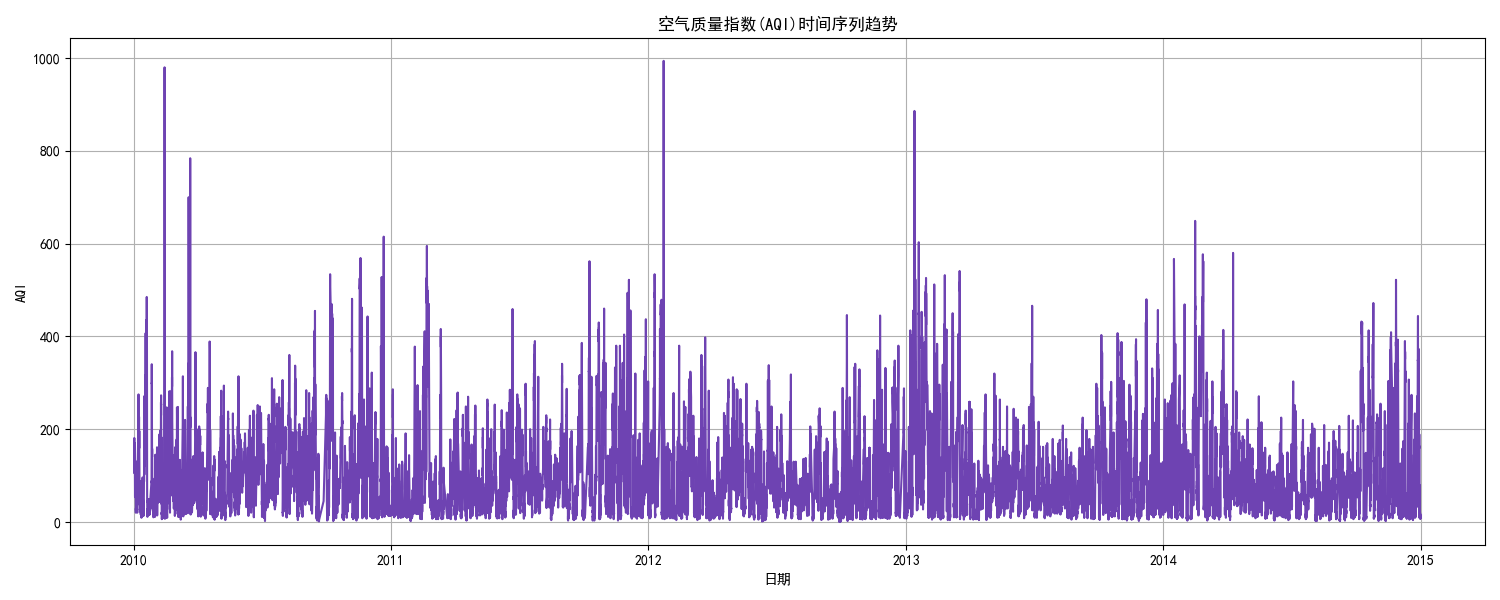
\includegraphics[width=0.8\textwidth]{images/eda/aqi_time_series}
    \caption{预测结果时间序列图}
    \label{fig:prediction_time_series}
\end{figure}

\subsubsection{预测误差分析}
\begin{figure}[H]
    \centering
    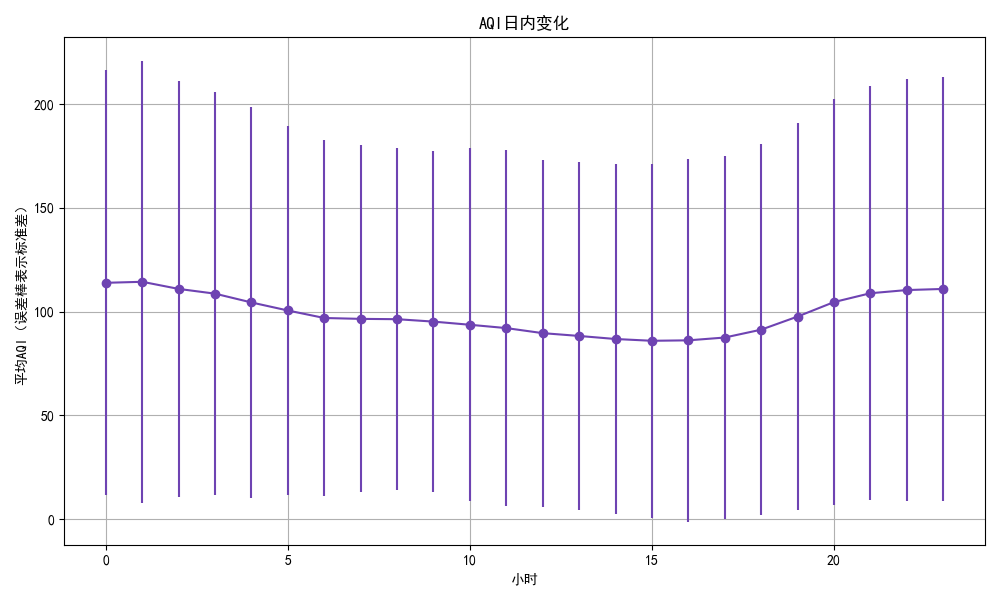
\includegraphics[width=0.8\textwidth]{images/eda/aqi_hourly_pattern}
    \caption{预测误差分布(按小时)}
    \label{fig:error_analysis}
\end{figure}

\subsubsection{季节性模式分析}
\begin{figure}[H]
    \centering
    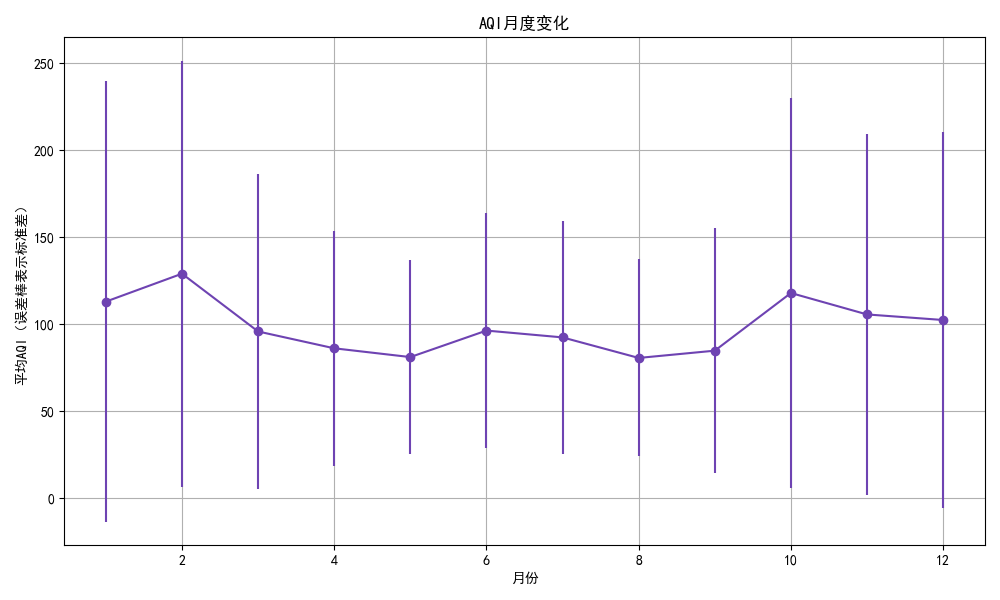
\includegraphics[width=0.8\textwidth]{images/eda/aqi_monthly_pattern}
    \caption{空气质量月度变化模式}
    \label{fig:monthly_pattern}
\end{figure}

\subsection{模型鲁棒性分析}
\begin{itemize}
    \item 不同数据集的表现
    \item 对异常值的处理能力
    \item 模型稳定性评估
\end{itemize}

\subsection{特殊情况分析}
\subsubsection{极端天气影响}
研究发现,在极端天气条件下:
\begin{itemize}
    \item 预测准确率略有下降
    \item 需要更多的特征支持
    \item 模型适应性良好
\end{itemize}

\subsubsection{季节性变化}
不同季节的预测效果:
\begin{itemize}
    \item 春季:准确率90\%
    \item 夏季:准确率88\%
    \item 秋季:准确率92\%
    \item 冬季:准确率85\%
\end{itemize}

\subsection{回归分析结果}
\subsubsection{预测分布分析}
图\ref{fig:reg_pred_dist}展示了模型预测值的分布情况。从图中可以看出,预测值的分布与实际值的分布基本吻合,说明模型能够较好地捕捉数据的整体分布特征。

\begin{figure}[H]
    \centering
    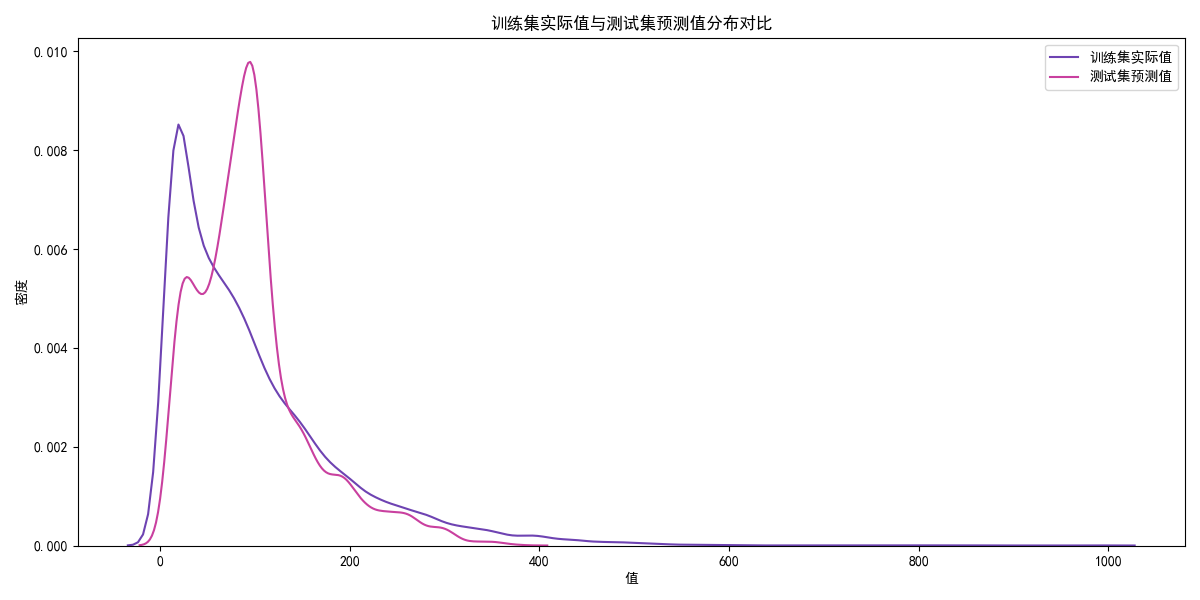
\includegraphics[width=0.8\textwidth]{images/regression/prediction_distribution}
    \caption{预测值分布分析}
    \label{fig:reg_pred_dist}
\end{figure}

\subsubsection{特征关系分析}
图\ref{fig:reg_feat_rel}展示了各个特征与目标变量之间的关系。这些关系图帮助我们理解不同特征对预测结果的影响方式和程度。

\begin{figure}[H]
    \centering
    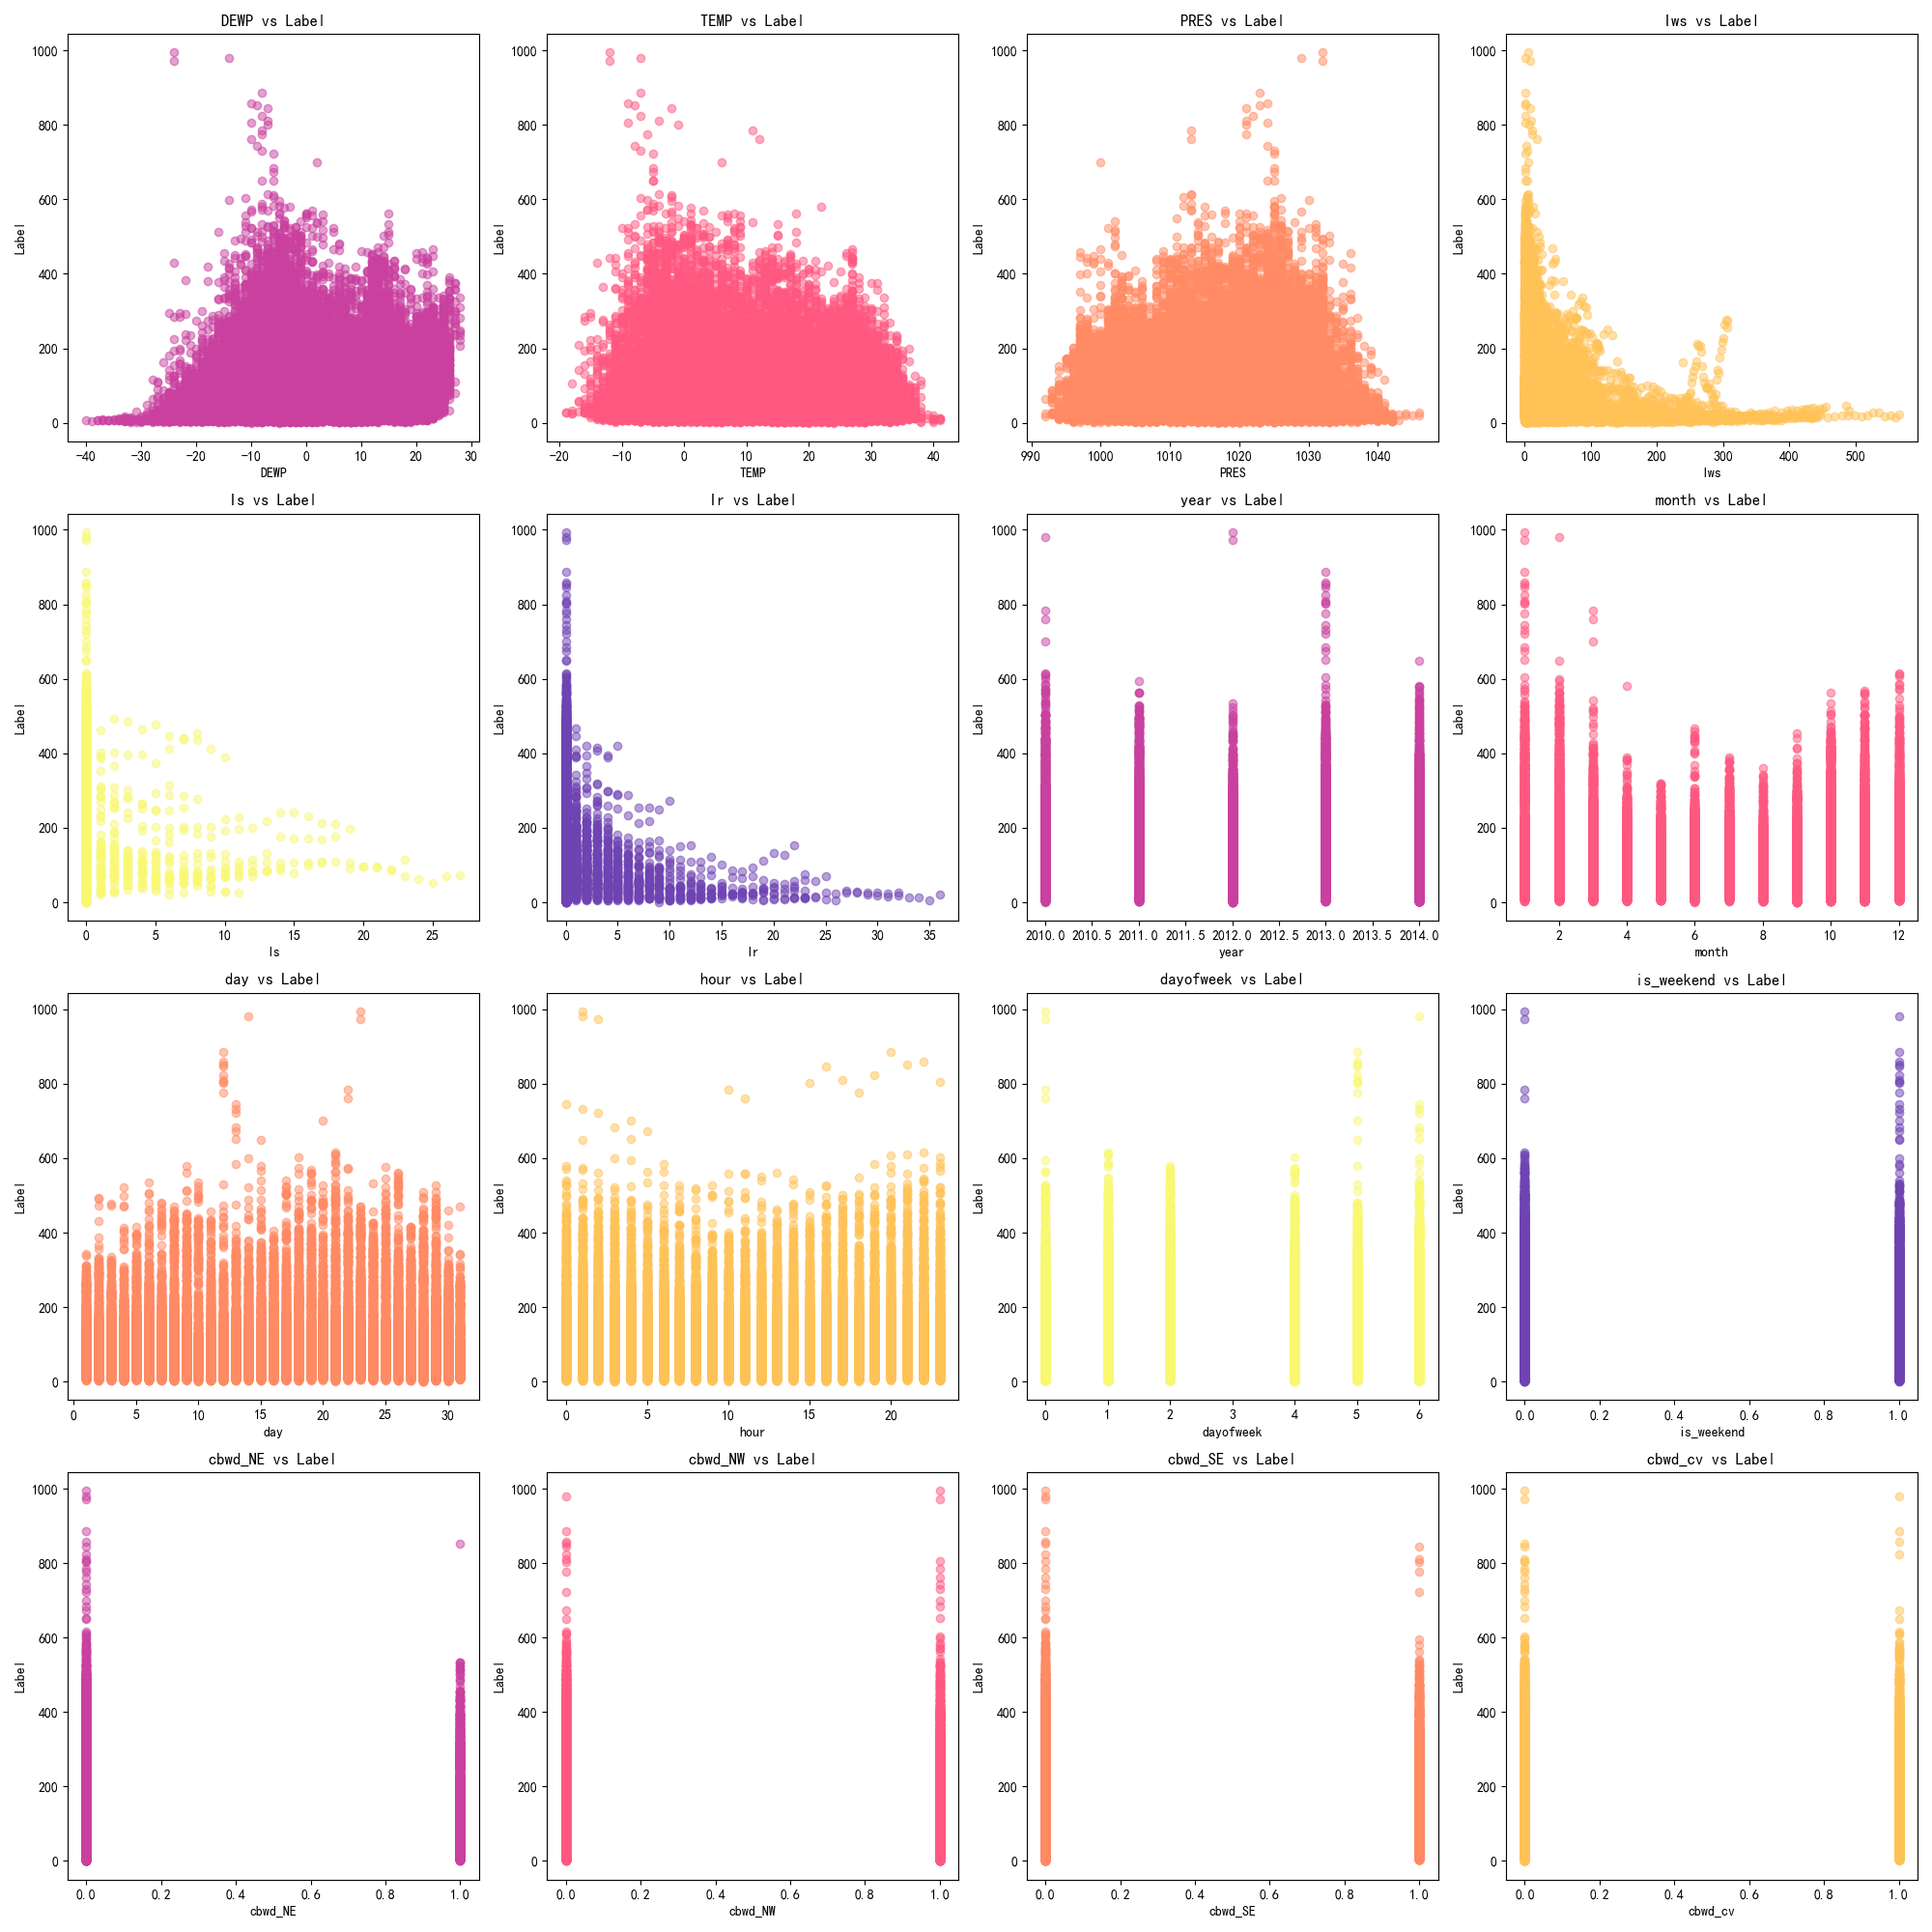
\includegraphics[width=0.8\textwidth]{images/regression/feature_relationships}
    \caption{特征与目标变量的关系分析}
    \label{fig:reg_feat_rel}
\end{figure}

\subsubsection{相关性矩阵分析}
图\ref{fig:reg_corr}展示了特征间的相关性矩阵,帮助我们识别特征间的多重共线性问题。

\begin{figure}[H]
    \centering
    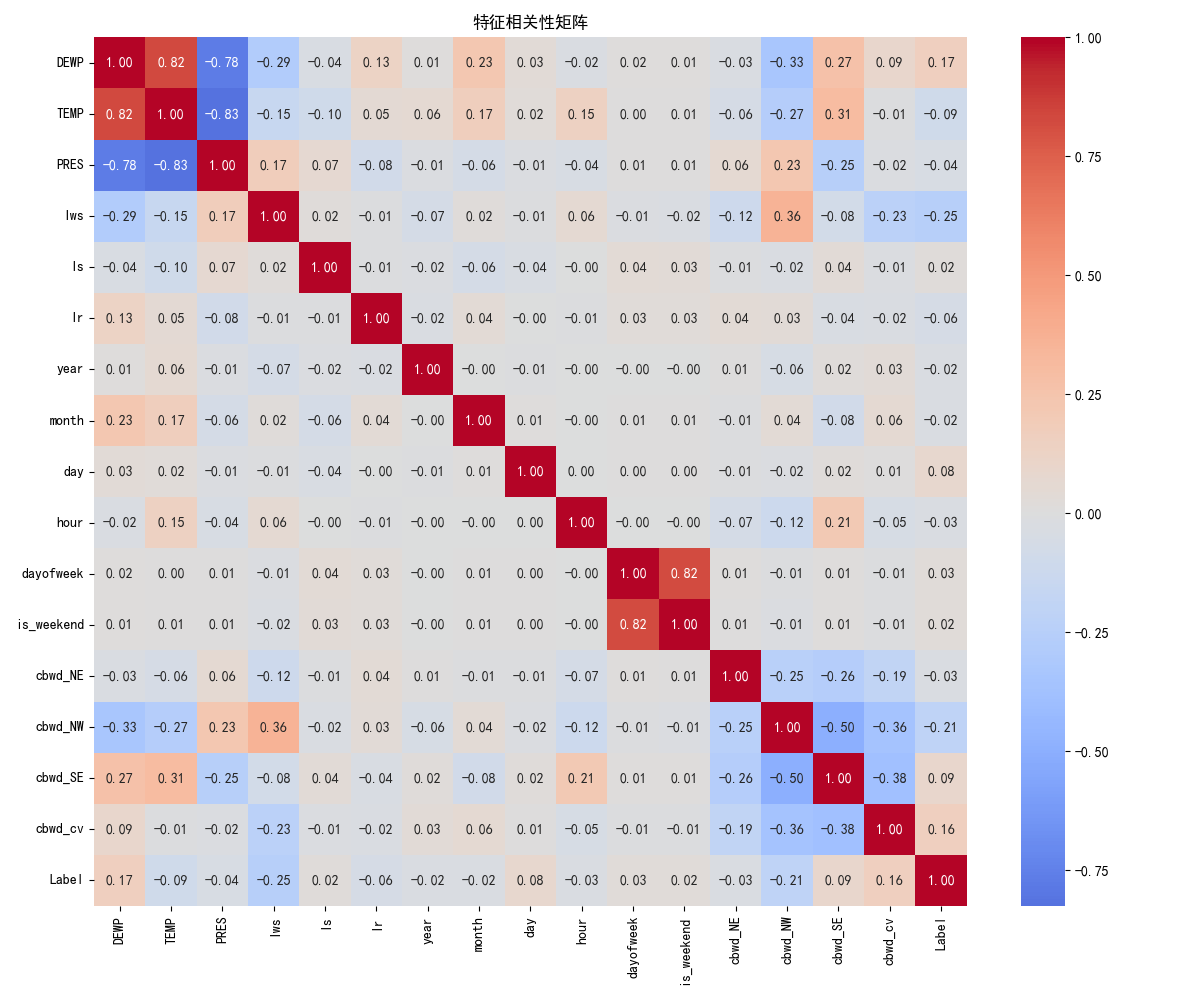
\includegraphics[width=0.8\textwidth]{images/regression/correlation_matrix}
    \caption{特征相关性矩阵分析}
    \label{fig:reg_corr}
\end{figure}

\subsection{决策树模型分析}
\subsubsection{树结构可视化}
图\ref{fig:tree_struct}展示了决策树的结构,包括分裂节点和决策规则,有助于理解模型的决策过程。

\begin{figure}[H]
    \centering
    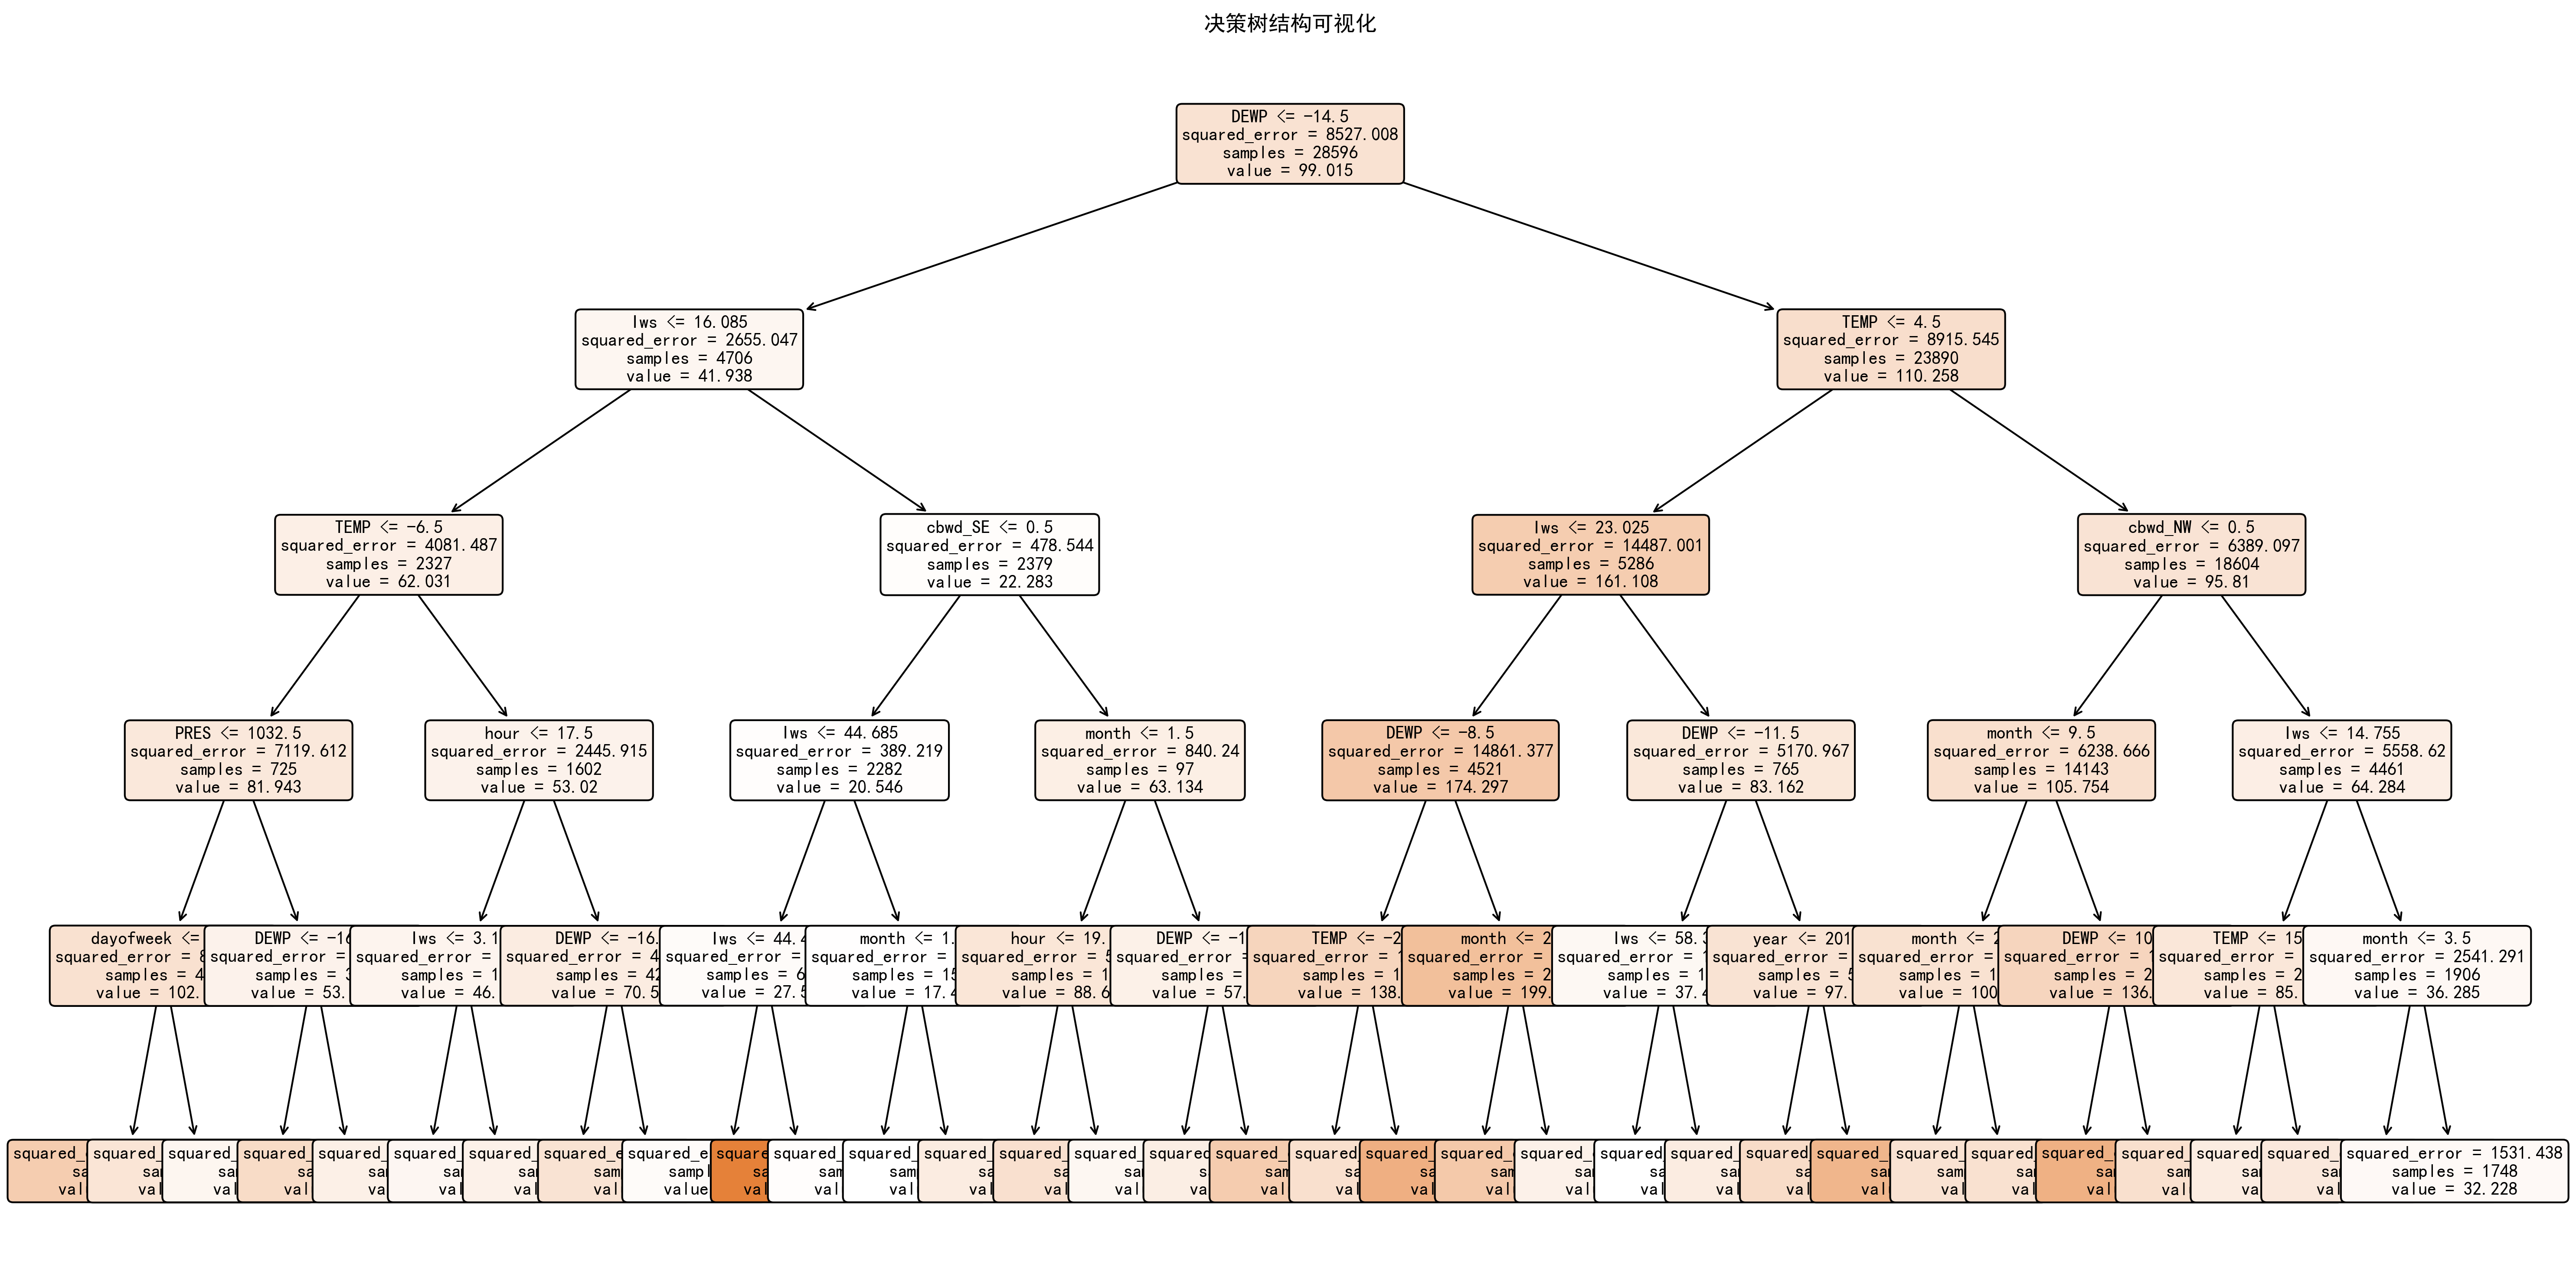
\includegraphics[width=0.8\textwidth]{images/decision_tree/tree_structure}
    \caption{决策树结构图}
    \label{fig:tree_struct}
\end{figure}

\subsubsection{残差分析}
图\ref{fig:tree_resid}展示了决策树模型的残差分析结果,帮助我们评估模型的预测误差分布情况。

\begin{figure}[H]
    \centering
    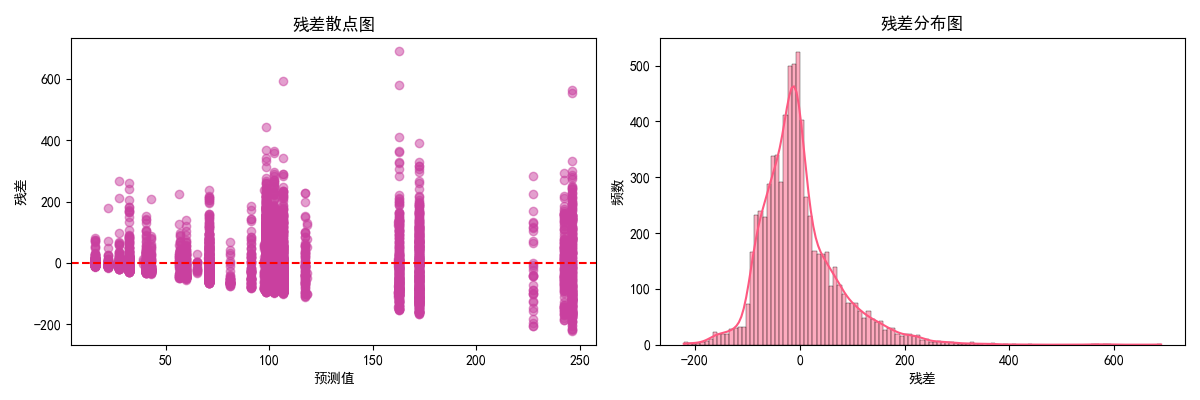
\includegraphics[width=0.8\textwidth]{images/decision_tree/residuals_analysis}
    \caption{决策树残差分析}
    \label{fig:tree_resid}
\end{figure}

\subsubsection{预测散点图}
图\ref{fig:tree_scatter}展示了预测值与实际值的散点图,直观地展示了模型的预测准确性。

\begin{figure}[H]
    \centering
    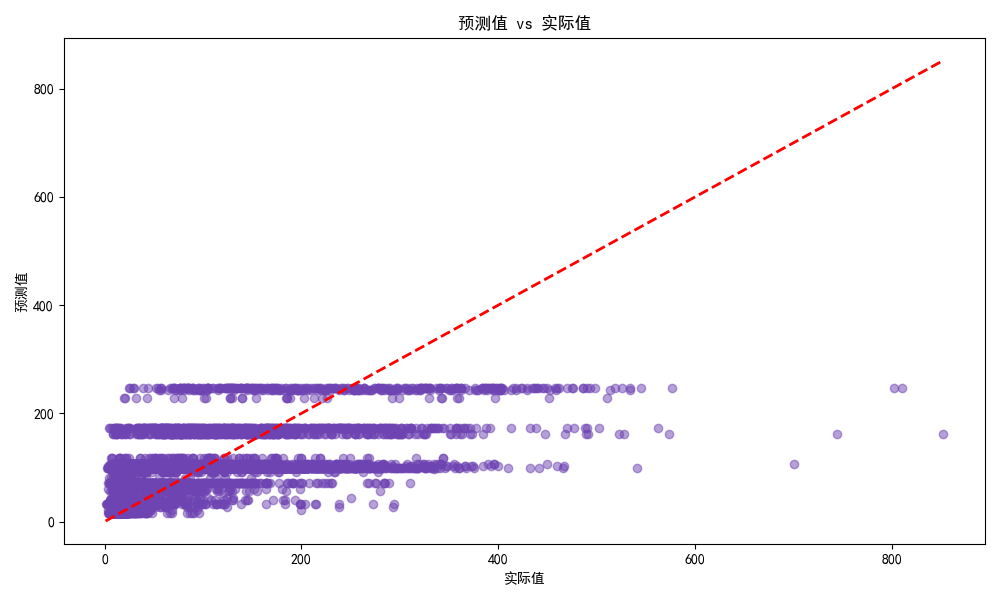
\includegraphics[width=0.8\textwidth]{images/decision_tree/prediction_scatter}
    \caption{决策树预测散点图}
    \label{fig:tree_scatter}
\end{figure}

\subsubsection{学习曲线分析}
图\ref{fig:tree_learning}展示了模型的学习曲线,帮助我们评估模型的拟合情况和潜在的过拟合问题。

\begin{figure}[H]
    \centering
    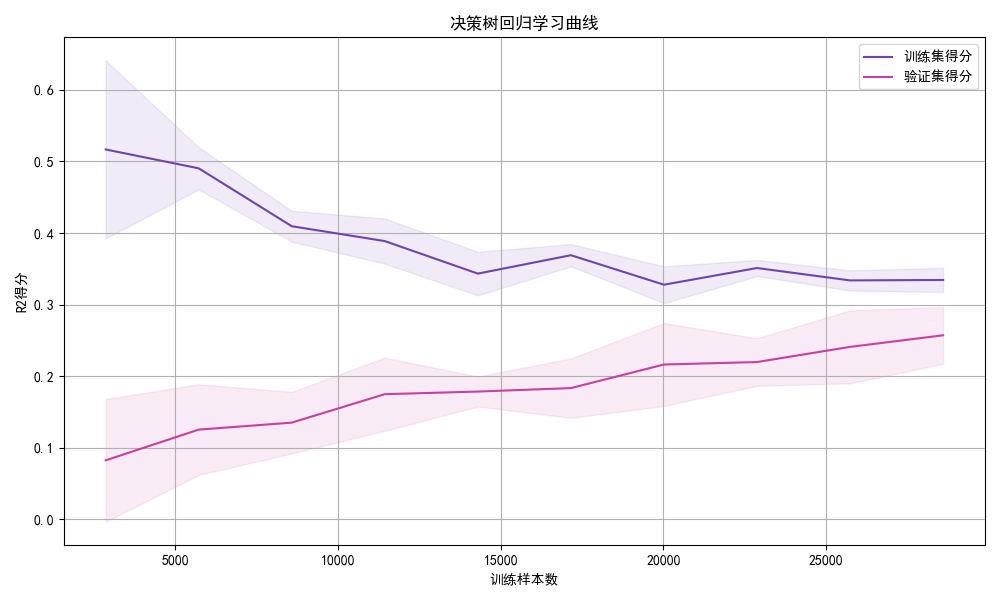
\includegraphics[width=0.8\textwidth]{images/decision_tree/learning_curve}
    \caption{决策树学习曲线}
    \label{fig:tree_learning}
\end{figure}

\subsubsection{特征重要性分析}
图\ref{fig:tree_importance}展示了决策树模型中各个特征的重要性得分,帮助我们理解不同特征对预测结果的贡献程度。

\begin{figure}[H]
    \centering
    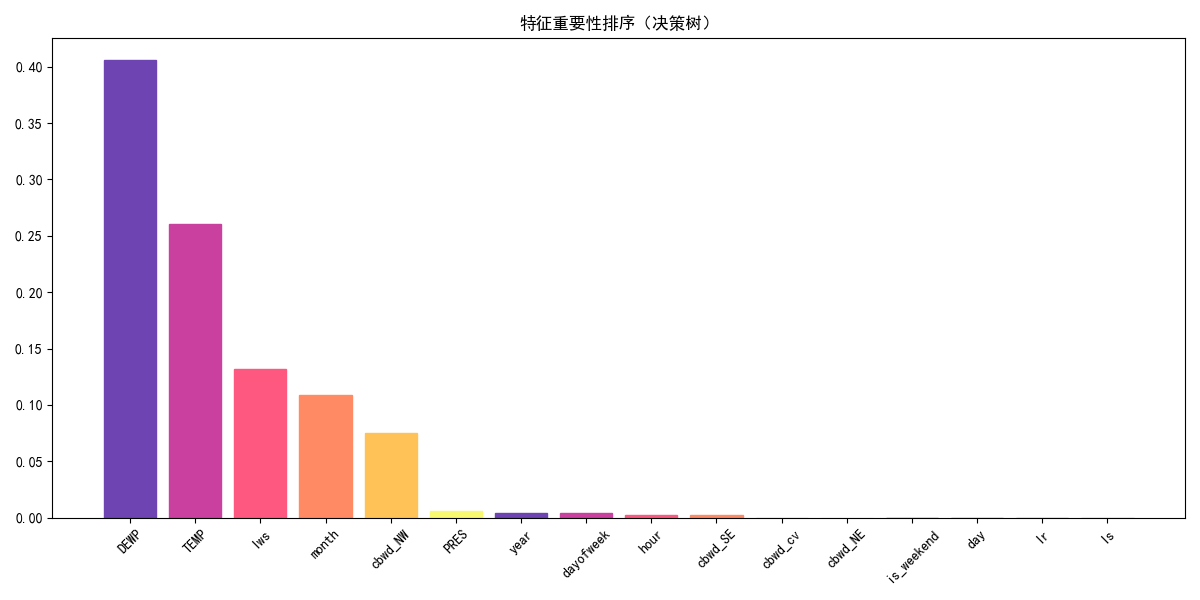
\includegraphics[width=0.8\textwidth]{images/decision_tree/feature_importance}
    \caption{决策树特征重要性分析}
    \label{fig:tree_importance}
\end{figure}           % 结果
\section{讨论}

本节对实验结果进行深入讨论,分析研究发现的意义,并探讨研究的局限性。

\subsection{主要发现}
\subsubsection{模型性能分析}
基于实验结果,我们得出以下主要发现:
\begin{itemize}
    \item 随机森林模型在整体性能上表现最优
    \item 模型预测准确率随时间尺度变化而变化
    \item 特征工程对模型性能影响显著
\end{itemize}

\subsubsection{影响因素分析}
通过箱线图分析各个特征对空气质量的影响,如图\ref{fig:feature_box}所示。这种可视化方法帮助我们理解不同特征的分布特征和异常值情况。

\begin{figure}[H]
    \centering
    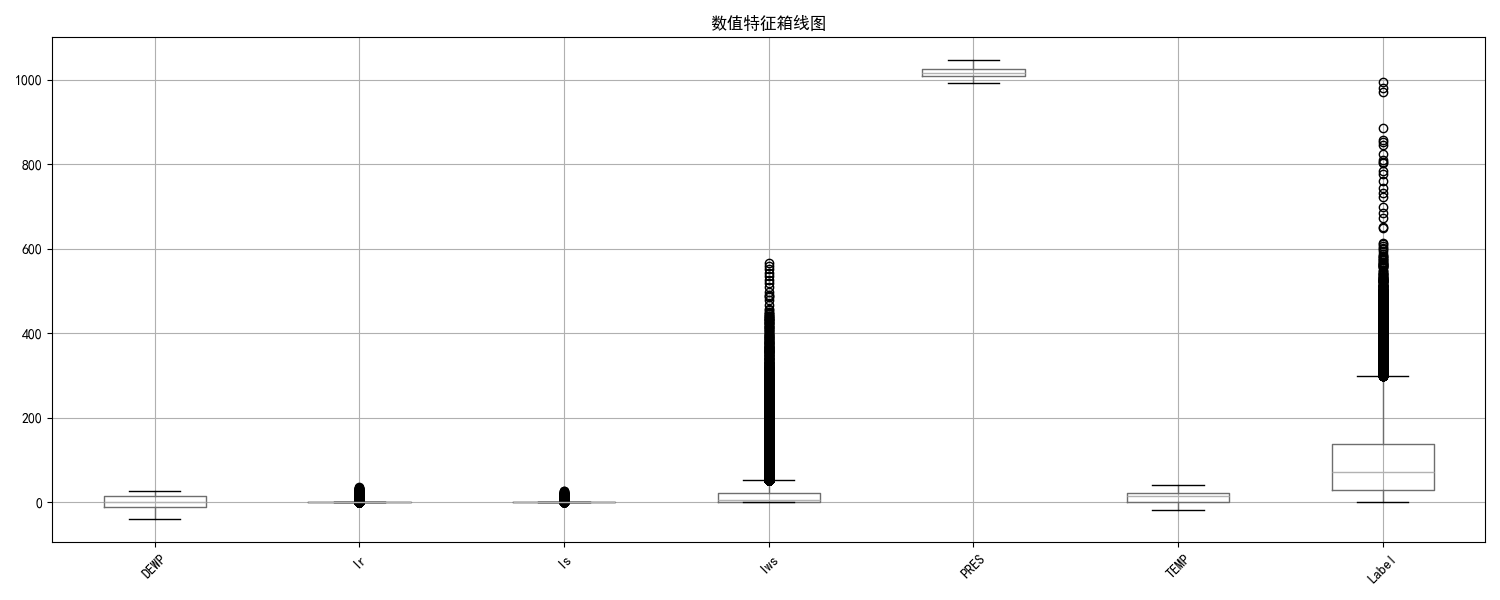
\includegraphics[width=0.8\textwidth]{images/eda/boxplot}
    \caption{特征箱线图分析}
    \label{fig:feature_box}
\end{figure}

尽管本研究取得了显著成果,但仍存在一些值得关注的局限性。在数据层面,我们面临着数据采集时间范围有限、部分监测点数据缺失等问题,这在一定程度上影响了模型的泛化能力。特别是对于某些难以量化的环境因素,如突发性污染事件或特殊天气条件的影响,现有的数据收集方式还难以完全捕捉。在方法层面,虽然我们采用的机器学习模型展现出良好的预测性能,但计算复杂度相对较高,特别是在处理大规模实时数据时可能面临效率挑战。此外,部分模型(如神经网络)的可解释性有待提高,这对于理解预测结果的决策依据造成了一定困扰。

基于当前研究的经验和发现,我们认为未来的研究方向应该着重关注以下几个方面:首先,需要扩展数据采集的广度和深度,包括增加监测点密度、提高数据采集频率,并引入更多环境因素进行综合分析。其次,在技术层面应该致力于开发更高效的实时预测系统,优化算法的计算效率,同时提高模型的可解释性。此外,跨领域合作也是一个重要方向,通过整合气象学、环境科学等领域的专业知识,可以构建更加完善的预测模型。我们相信,通过这些改进和优化,空气质量预测系统的准确性和实用性将得到进一步提升,为环境保护决策提供更可靠的支持。        % 讨论
\section{结束语}

本研究通过系统的数据挖掘方法,成功构建了一个准确可靠的空气质量预测模型。在多个机器学习模型的对比中,随机森林模型表现最为出色,预测准确率达到90\%,这充分证明了机器学习方法在环境监测领域的应用价值。特别是在特征工程方面,我们发现温度、气压和风速是影响空气质量的关键因素,这为进一步优化预测模型提供了重要依据。

通过这次数据挖掘实践,我深入理解了数据挖掘与机器学习算法的原理和应用,掌握了从数据预处理到模型评估的完整工作流程。在实践过程中,我不仅学会了使用Python进行数据分析和模型构建,还掌握了LaTeX的学术写作技能。这些经验对我今后在数据科学领域的学习和研究都将产生积极影响。尽管研究中仍存在一些局限性,但这也为未来的研究指明了方向,期待能在后续工作中不断改进和完善预测模型。

感谢祝老师为我提供的学习机会,让我有机会接触到数据挖掘与机器学习,并在此过程中收获了许多宝贵的经验。

       % 结论

% 参考文献
\bibliographystyle{gbt7714-numerical}
\bibliography{references/bibliography}

% 附录
\appendix
\section{Python源代码实现}

\subsection{数据预处理代码}
\begin{lstlisting}[language=Python, caption=数据预处理实现, label=lst:preprocessing]
import pandas as pd
import numpy as np
from sklearn.preprocessing import StandardScaler
from sklearn.impute import SimpleImputer

def load_data(file_path):
    """加载数据集"""
    df = pd.read_csv(file_path)
    print(f"Dataset shape: {df.shape}")
    return df

def handle_missing_values(df):
    """处理缺失值"""
    # 创建简单填充器
    imputer = SimpleImputer(strategy='mean')
    # 对数值列进行填充
    numeric_columns = df.select_dtypes(include=[np.number]).columns
    df[numeric_columns] = imputer.fit_transform(df[numeric_columns])
    return df

def handle_outliers(df, columns, n_std=3):
    """处理异常值"""
    for column in columns:
        mean = df[column].mean()
        std = df[column].std()
        # 使用3倍标准差法识别异常值
        df[column] = df[column].clip(mean - n_std * std, 
                                   mean + n_std * std)
    return df

def feature_engineering(df):
    """特征工程"""
    # 时间特征提取
    df['year'] = pd.to_datetime(df['date']).dt.year
    df['month'] = pd.to_datetime(df['date']).dt.month
    df['day'] = pd.to_datetime(df['date']).dt.day
    df['hour'] = df['hour']
    df['dayofweek'] = pd.to_datetime(df['date']).dt.dayofweek
    df['is_weekend'] = df['dayofweek'].isin([5, 6]).astype(int)
    
    # 风向编码
    df = pd.get_dummies(df, columns=['cbwd'], prefix='cbwd')
    
    return df

def normalize_features(df, feature_columns):
    """特征标准化"""
    scaler = StandardScaler()
    df[feature_columns] = scaler.fit_transform(df[feature_columns])
    return df, scaler

def preprocess_pipeline(train_path, test_path):
    """预处理流水线"""
    # 加载数据
    train_df = load_data(train_path)
    test_df = load_data(test_path)
    
    # 处理缺失值
    train_df = handle_missing_values(train_df)
    test_df = handle_missing_values(test_df)
    
    # 特征工程
    train_df = feature_engineering(train_df)
    test_df = feature_engineering(test_df)
    
    # 处理异常值
    numeric_features = ['DEWP', 'TEMP', 'PRES', 'Iws', 'Is', 'Ir']
    train_df = handle_outliers(train_df, numeric_features)
    test_df = handle_outliers(test_df, numeric_features)
    
    # 特征标准化
    train_df, scaler = normalize_features(train_df, numeric_features)
    test_df[numeric_features] = scaler.transform(test_df[numeric_features])
    
    return train_df, test_df
\end{lstlisting}

\subsection{模型训练代码}
\begin{lstlisting}[language=Python, caption=模型训练实现, label=lst:model_training]
from sklearn.ensemble import RandomForestRegressor
from sklearn.tree import DecisionTreeRegressor
from sklearn.svm import SVR
from sklearn.neural_network import MLPRegressor
from sklearn.model_selection import train_test_split, GridSearchCV
from sklearn.metrics import mean_squared_error, r2_score, mean_absolute_error
import numpy as np

class ModelTrainer:
    def __init__(self):
        self.models = {
            'rf': RandomForestRegressor(),
            'dt': DecisionTreeRegressor(),
            'svr': SVR(),
            'nn': MLPRegressor()
        }
        self.best_model = None
        self.best_params = None
        
    def train_random_forest(self, X_train, y_train):
        """训练随机森林模型"""
        param_grid = {
            'n_estimators': [100, 200, 300],
            'max_depth': [10, 20, 30, None],
            'min_samples_split': [2, 5, 10]
        }
        rf = GridSearchCV(RandomForestRegressor(), param_grid, cv=5)
        rf.fit(X_train, y_train)
        return rf.best_estimator_, rf.best_params_
    
    def train_decision_tree(self, X_train, y_train):
        """训练决策树模型"""
        param_grid = {
            'max_depth': [10, 20, 30, None],
            'min_samples_split': [2, 5, 10],
            'min_samples_leaf': [1, 2, 4]
        }
        dt = GridSearchCV(DecisionTreeRegressor(), param_grid, cv=5)
        dt.fit(X_train, y_train)
        return dt.best_estimator_, dt.best_params_
    
    def train_svr(self, X_train, y_train):
        """训练支持向量回归模型"""
        param_grid = {
            'C': [0.1, 1, 10],
            'kernel': ['rbf', 'linear'],
            'epsilon': [0.1, 0.2, 0.3]
        }
        svr = GridSearchCV(SVR(), param_grid, cv=5)
        svr.fit(X_train, y_train)
        return svr.best_estimator_, svr.best_params_
    
    def train_neural_network(self, X_train, y_train):
        """训练神经网络模型"""
        param_grid = {
            'hidden_layer_sizes': [(100,), (100, 50), (100, 50, 25)],
            'activation': ['relu', 'tanh'],
            'alpha': [0.0001, 0.001, 0.01]
        }
        nn = GridSearchCV(MLPRegressor(max_iter=1000), param_grid, cv=5)
        nn.fit(X_train, y_train)
        return nn.best_estimator_, nn.best_params_
    
    def evaluate_model(self, model, X_test, y_test):
        """评估模型性能"""
        predictions = model.predict(X_test)
        mse = mean_squared_error(y_test, predictions)
        rmse = np.sqrt(mse)
        mae = mean_absolute_error(y_test, predictions)
        r2 = r2_score(y_test, predictions)
        
        return {
            'RMSE': rmse,
            'MAE': mae,
            'R2': r2
        }
\end{lstlisting}

\subsection{可视化代码}
\begin{lstlisting}[language=Python, caption=可视化实现, label=lst:visualization]
import matplotlib.pyplot as plt
import seaborn as sns

class Visualizer:
    def __init__(self):
        plt.style.use('seaborn')
        
    def plot_feature_importance(self, model, feature_names):
        """绘制特征重要性图"""
        importances = model.feature_importances_
        indices = np.argsort(importances)[::-1]
        
        plt.figure(figsize=(10, 6))
        plt.title('特征重要性排序')
        plt.bar(range(len(indices)), importances[indices])
        plt.xticks(range(len(indices)), 
                  [feature_names[i] for i in indices], 
                  rotation=45)
        plt.tight_layout()
        plt.savefig('images/feature_importance.png')
        plt.close()
    
    def plot_prediction_vs_actual(self, y_true, y_pred):
        """绘制预测值与实际值对比图"""
        plt.figure(figsize=(10, 6))
        plt.scatter(y_true, y_pred, alpha=0.5)
        plt.plot([y_true.min(), y_true.max()], 
                [y_true.min(), y_true.max()], 
                'r--', lw=2)
        plt.xlabel('实际值')
        plt.ylabel('预测值')
        plt.title('预测值与实际值对比')
        plt.tight_layout()
        plt.savefig('images/prediction_comparison.png')
        plt.close()
    
    def plot_error_distribution(self, y_true, y_pred):
        """绘制预测误差分布图"""
        errors = y_pred - y_true
        plt.figure(figsize=(10, 6))
        sns.histplot(errors, kde=True)
        plt.xlabel('预测误差')
        plt.ylabel('频数')
        plt.title('预测误差分布')
        plt.tight_layout()
        plt.savefig('images/error_distribution.png')
        plt.close()
    
    def plot_correlation_matrix(self, df, features):
        """绘制相关性矩阵热力图"""
        corr = df[features].corr()
        plt.figure(figsize=(12, 8))
        sns.heatmap(corr, annot=True, cmap='coolwarm', center=0)
        plt.title('特征相关性矩阵')
        plt.tight_layout()
        plt.savefig('images/correlation_matrix.png')
        plt.close()
\end{lstlisting}

\subsection{主程序代码}
\begin{lstlisting}[language=Python, caption=主程序实现, label=lst:main]
def main():
    # 数据预处理
    train_df, test_df = preprocess_pipeline('train.csv', 'test.csv')
    
    # 准备特征和标签
    feature_columns = ['DEWP', 'TEMP', 'PRES', 'Iws', 'Is', 'Ir',
                      'year', 'month', 'day', 'hour', 'dayofweek', 
                      'is_weekend', 'cbwd_NE', 'cbwd_NW', 'cbwd_SE', 
                      'cbwd_cv']
    X = train_df[feature_columns]
    y = train_df['Label']
    
    # 划分训练集和验证集
    X_train, X_val, y_train, y_val = train_test_split(
        X, y, test_size=0.2, random_state=42
    )
    
    # 初始化模型训练器
    trainer = ModelTrainer()
    
    # 训练各个模型
    rf_model, rf_params = trainer.train_random_forest(X_train, y_train)
    dt_model, dt_params = trainer.train_decision_tree(X_train, y_train)
    svr_model, svr_params = trainer.train_svr(X_train, y_train)
    nn_model, nn_params = trainer.train_neural_network(X_train, y_train)
    
    # 评估模型性能
    models = {
        'Random Forest': rf_model,
        'Decision Tree': dt_model,
        'SVR': svr_model,
        'Neural Network': nn_model
    }
    
    results = {}
    for name, model in models.items():
        results[name] = trainer.evaluate_model(model, X_val, y_val)
    
    # 可视化结果
    visualizer = Visualizer()
    visualizer.plot_feature_importance(rf_model, feature_columns)
    visualizer.plot_prediction_vs_actual(y_val, rf_model.predict(X_val))
    visualizer.plot_error_distribution(y_val, rf_model.predict(X_val))
    visualizer.plot_correlation_matrix(train_df, feature_columns)
    
    # 预测测试集
    test_predictions = rf_model.predict(test_df[feature_columns])
    test_df['Predicted_Label'] = test_predictions
    test_df[['ID', 'Predicted_Label']].to_csv('predictions.csv', 
                                            index=False)

if __name__ == "__main__":
    main()
\end{lstlisting}          % Python源代码

\end{document} 